\documentclass[a4paper,english,12pt]{article}
\usepackage{etex}
\usepackage{graphicx}
\usepackage{epstopdf}
\usepackage{amsmath}
\usepackage{%
	amsfonts,%
	amsmath,%	
	amssymb,%
	amsthm,%
	algorithm,%
	babel,%
	bbm,%
	etex,%
	%biblatex,%
	caption,%
	centernot,%
	color,%
	dsfont,%
	enumerate,%
	epsfig,%
	epstopdf,%
	geometry,%
	graphicx,%
	hyperref,%
	latexsym,%
	mathtools,%
	multicol,%
	pgf,%
	pgfplots,%
	pgfplotstable,%
	pgfpages,%
	proof,%
	psfrag,%
	subfigure,%	
	tikz,%
	ulem,%
	url%
}	
\usepackage[noend]{algpseudocode}
\usepackage[mathscr]{eucal}
\usepgflibrary{shapes}
\usetikzlibrary{%
  	arrows,%
	backgrounds,%
	chains,%
	decorations.pathmorphing,% /pgf/decoration/random steps | erste Graphik
	decorations.text,%
	matrix,%
  	positioning,% wg. " of "
  	fit,%
	patterns,%
  	petri,%
	plotmarks,%
  	scopes,%
	shadows,%
  	shapes.misc,% wg. rounded rectangle
  	shapes.arrows,%
	shapes.callouts,%
  	shapes%
}

\theoremstyle{plain}
\newtheorem{thm}{Theorem}[section]
\newtheorem{lem}[thm]{Lemma}
\newtheorem{prop}[thm]{Proposition}
\newtheorem{cor}[thm]{Corollary}

\theoremstyle{definition}
\newtheorem{defn}[thm]{Definition}
\newtheorem{conj}[thm]{Conjecture}
\newtheorem{exmp}[thm]{Example}
\newtheorem{assum}[thm]{Assumptions}
\newtheorem{axiom}[thm]{Axiom}

\theoremstyle{remark}
\newtheorem{rem}{Remark}
\newtheorem{note}{Note}
\newtheorem{fact}{Fact}

\newcommand{\norm}[1]{\left\lVert#1\right\rVert}
\newcommand{\indep}{\!\perp\!\!\!\perp}
\DeclarePairedDelimiter\abs{\lvert}{\rvert}%
\newcommand\numberthis{\addtocounter{equation}{1}\tag{\theequation}}
\newcommand{\tr}{\operatorname{tr}}
\newcommand{\R}{\mathbb{R}}
\newcommand{\N}{\mathbb{N}}
\newcommand{\E}{\mathbb{E}}
\newcommand{\Z}{\mathbb{Z}}
\newcommand{\B}{\mathscr{B}}
\newcommand{\C}{\mathcal{C}}
\newcommand{\T}{\mathscr{T}}
\newcommand{\F}{\mathcal{F}}
\newcommand{\G}{\mathcal{G}}
%\newcommand{\ba}{\begin{align*}}
%\newcommand{\ea}{\end{align*}}
\DeclareMathOperator*{\argmax}{arg\,max}
\renewcommand{\qedsymbol}{$\blacksquare$}
\makeatletter
\def\BState{\State\hskip-\ALG@thistlm}
\makeatother

\makeatletter
\def\th@plain{%
  \thm@notefont{}% same as heading font
  \itshape % body font
}
\def\th@definition{%
  \thm@notefont{}% same as heading font
  \normalfont % body font
}
\makeatother
\date{}

%opening
\title{Lecture 2: Minimax Hypothesis}
\date{14 Jan 16}

\begin{document}
\maketitle

\section{Continued from the Lecture 1}
At the onset, we will look into two examples of Bayesian Hypothesis Testing which was covered in Lecture 1.  

\begin{exmp}[The Binary Channel] 
A binary channel is a common communication channel model used in coding theory and information theory. In this model, a transmitter wishes to send a bit (a zero or a one), and the receiver receives a bit, again zero or one. The bit may be transmitted correctly with some probability, or it may be "flipped" with the same or some different probability (the "crossover probability").\\ 
Say on such a Binary Communication Channel a binary digit is to be transmitted. Our observation Y is the output of the channel, which can also be either zero or one. A transmitted "zero" is received as a "one" with probability $\lambda_0$ and as a "zero" with probability (1 - $\lambda_0$), where $0 \leq \lambda_0 \leq 1$. Similarly, a transmitted "one" is received as a "zero" with probability $\lambda_1$ and as a "one" with probability (1- $\lambda_1$). In case $\lambda_0=\lambda_1=\lambda$, then the channel is said to be a Binary Symmetric Channel (BSC). Thus, only observing Y does not tell us exactly whether the transmitted digit was a "zero" or a "one". Our aim is to find an optimum decision rule using the Bayesian Hypothesis Testing.

\begin{figure}[h]
\centering
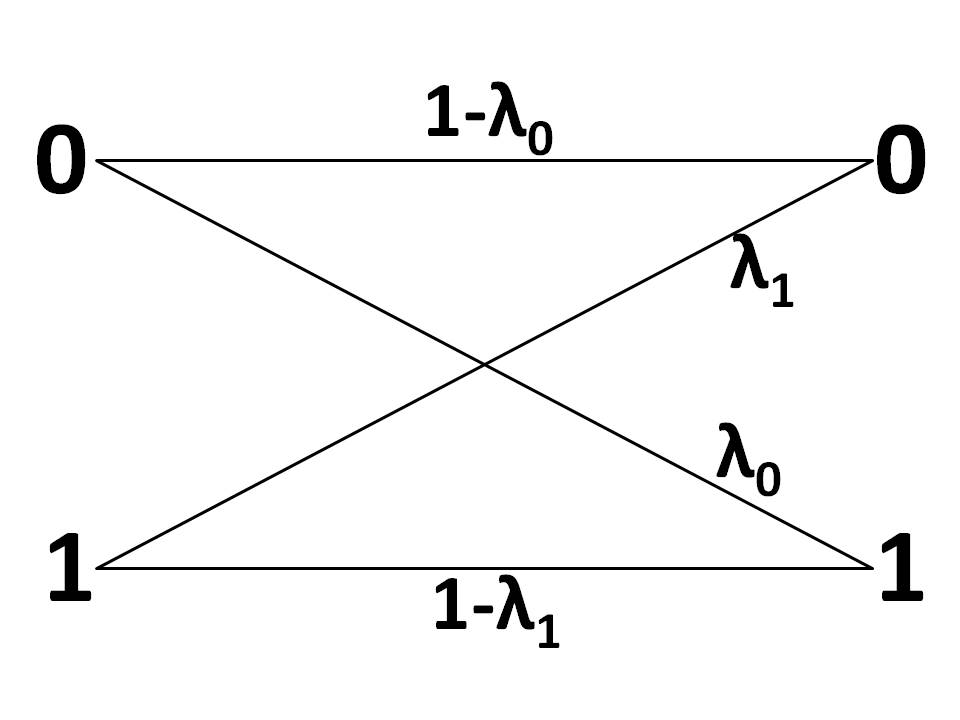
\includegraphics[width=0.7\linewidth]{Figures/bsc1}
\caption{Block diagram for Binary Channel}
\label{fig:bsc1}
\end{figure}

This situation can be seen as a Bayesian Hypothesis Testing problem with the two hypothesis $ H_0~ and~ H_1 $ depicted as transmission of a "zero" and transmission of a "one" respectively. The observation set is $\Gamma$ \{0,1\}. The recieved signal $Y \in \Gamma$  will have a Bernoulli PDF as follows:\\
\begin{eqnarray}
Y_{0}~\sim~\left( 1-\lambda_{0}\right) ~if~H_0~is~transmitted\\
Y_{1}~\sim~\left( 1-\lambda_{1}\right)~if~H_1~is~transmitted \end{eqnarray}
and the observation Y has densities (i.e., probability mass functions):
\begin{equation}
p_{j}\left( y\right) = \lambda_{j} ,~if~ y\neq j,
\end{equation}
\begin{equation}
p_{j}\left( y\right) = \left( 1-\lambda_{j}\right),~if~ y=j
\end{equation}
for $j \in \{0,1\}$.
The likelihood ratio will then be given by \\
\begin{eqnarray}
L(y) = \frac{p_1(y)}{p_0(y)} = \frac{\lambda_1}{1-\lambda_0} ~~~~~~~if~ y=0 \\
L(y) = \frac{p_1(y)}{p_0(y)} = \frac{1-\lambda_1}{\lambda_0} ~~~~~~~if~ y=1
\end{eqnarray}

To calculate the threshold $\tau= \frac{\pi_0(C_{10}-C_{00})}{\pi_1(C_{01}-C_{11})}$, we need the priors and the costs. \\
If $\lambda_0,~\lambda_1,~\tau$  are such that $\lambda_1\geq \tau\left( 1-\lambda_0\right) $, then the probability of a flip is higher and hence the likelihood ratio decides a recieved 0 as a transmitted 1 and vice versa.\\
Based on this likelihood function, we will derive the decision rule. Let us take the simple case of uniform cost, in which $C_{ij} = 0~ if~ i=j~ and~ C_{ij} = 1~ if ~i\neq j$. In this case, the Bayesian decision rule is given as follows:\\
\begin{eqnarray}
\delta_{B}(0)=1~if~(1-\lambda_1)<\lambda_0\\ 
\delta_{B}(0)=0~if~(1-\lambda_1)\geq\lambda_0
\end{eqnarray}
\begin{eqnarray}
\delta_{B}(1)=1~if~(1-\lambda_1)\geq\lambda_0\\
\delta_{B}(1)=0~if~(1-\lambda_1)<\lambda_0
\end{eqnarray}

Generally speaking,\\
\begin{equation}
\delta_{B}(y)=y,~if~(1-\lambda_1)\geq\lambda_0
\end{equation}
\begin{equation}
~~~~~~~\delta_{B}(y)=\left( 1-y\right), ~if~(1-\lambda_1)<\lambda_0
\end{equation}

Under symmetric channel condition $(\lambda_1=\lambda_0=\lambda)$,
\begin{equation}
\delta_{B}(y)=y,~if~\lambda< 0.5\\
\end{equation}
\begin{equation}
~~~~~~~~\delta_{B}(y)=\left( 1-y\right), ~if~\lambda\geq0.5
\end{equation}
Now, under this decision rule, we will look into the unconditional risk. Under uniform cost condition, 

\begin{align}
R_0(\delta)&=\lambda_0~~~~~~~~~~~if~(1-\lambda_1)\geq\lambda_0 \\
&=\left( 1-\lambda_0\right)~~~if~(1-\lambda_1)<\lambda_0
\end{align}
\begin{align}
R_1(\delta)&=\lambda_1~~~~~~~~~~~if~(1-\lambda_1)\geq\lambda_0 \\
&=\left( 1-\lambda_1\right)~~~if~(1-\lambda_1)<\lambda_0
\end{align}

Under symmetric channel condition, it turns out to be 

\centering
\begin{equation}
r(\delta)= min\left( \lambda,1-\lambda\right)
\end{equation}
\end{exmp}

\begin{exmp}[Location Testing with Gaussian Error] 
Let us consider the typical communication model  denoted by the equation 

\begin{equation}
y=x+h
\end{equation}
\begin{figure}[h]
\centering
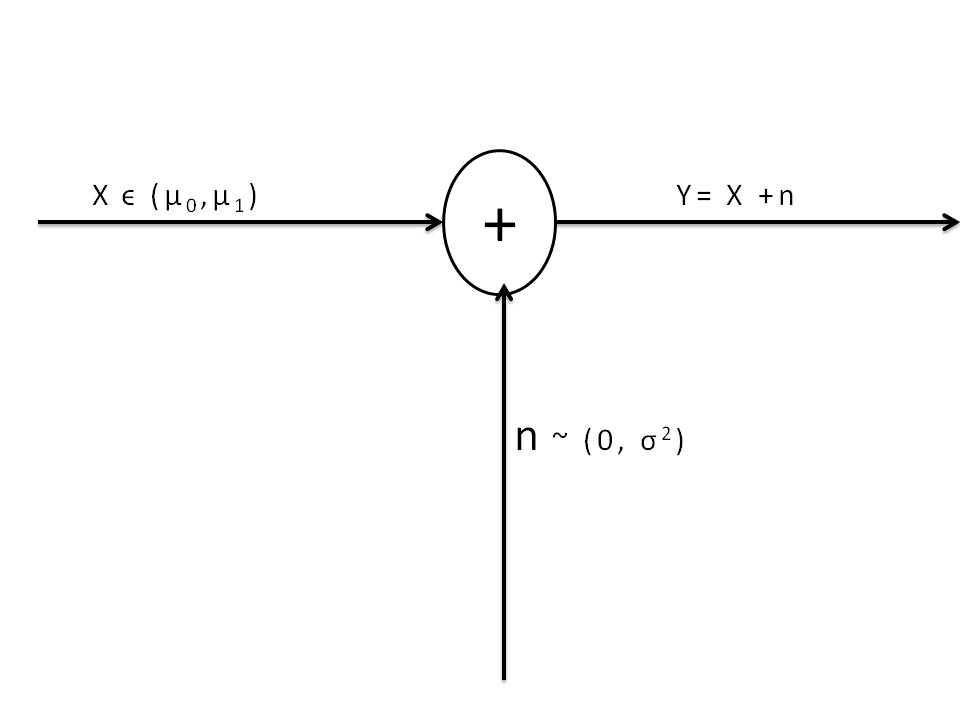
\includegraphics[width=0.7\linewidth]{Figures/AWGN}
\caption[awgn]{AWGN channel}
\label{fig:AWGN}
\end{figure}
In this example the Null Hypothesis $(H_0)$ indicates transmission of Signal with mean $\mu_0$ and alternative Hypothesis $(H_1)$ indicates transmission of Signal with mean $\mu_1$. Hence the received signal y will have a PDF as follows:\\
\begin{eqnarray}
{H_0}~:y \sim \mathcal{N} \left( \mu _0, \sigma^2\right) \\
{H_1}:y \sim \mathcal{N} \left( \mu _1, \sigma^2\right)
\end{eqnarray}
and the observation space will be $\Gamma \in \mathcal{R}$. For uniform cost, equal priors and $\mu_1>\mu_0,$\\
\begin{equation}
L(y) = \frac{{{P_1}(y)}}{{{P_0}(y)}} = \frac{{\frac{1}{{\sigma \sqrt {2\pi } }}e\frac{{ - {{(y - {\mu _1})}^2}}}{{2{\sigma ^2}}}}}{{\frac{1}{{\sigma \sqrt {2\pi } }}e\frac{{ - {{(y - {\mu _0})}^2}}}{{2{\sigma ^2}}}}}
\end{equation}

\begin{equation}
~~~~~~~~~~~~~~~~~~~~~={e^{\frac{{[ - {{(y - {\mu _1})}^2} + {{(y - {\mu _0})}^2}}}{{2{\sigma ^2}}}}}
\end{equation}
\begin{equation}
	~~~~~~~~~~~~~~~={e^{\frac{{({\mu _{1 - }}{\mu _0})\left( {y - (\frac{{{\mu _{1 + }}{\mu _0}}}{2})} \right)}}{{{\sigma ^2}}}}}
\end{equation}
For uniform cost and equal priors, $\tau = 1$ and $\Gamma_1 = {L(y)\geq1}$.\\ Hence for 
\begin{equation}
	{e^{\frac{{({\mu _{1 - }}{\mu _0})\left( {y - (\frac{{{\mu _{1 + }}{\mu _0}}}{2})} \right)}}{{{\sigma ^2}}}}}\geq 1,
\end{equation}
\begin{equation}
	{\frac{{({\mu _{1 - }}{\mu _0})\left( {y - (\frac{{{\mu _{1 + }}{\mu _0}}}{2})} \right)}}{{{\sigma ^2}}}}\geq 0
\end{equation}
Therefore,
\begin{equation}
{~~~~~~~~~~~~~~~\Gamma _1} = \{ \frac{{{\mu _1} - {\mu _0}}}{{{\sigma ^2}}}(y - \frac{{({\mu _1} + {\mu _0})}}{2})\}\geq0 \\
\end{equation}
\begin{equation}
=\{ y \ge \frac{{{\mu _1} + {\mu _0}}}{2}\}
\end{equation}
Thus the decision rule in this case will be\\
\begin{equation}
\delta(y)= 1 ~ if~ \{ y \ge \frac{{{\mu _1} + {\mu _0}}}{2}\}
\end{equation}
\begin{equation}
\delta(y)= 0 ~ if~ \{ y < \frac{{{\mu _1} + {\mu _0}}}{2}\}
\end{equation}
The conditional risk is given by\\
\begin{eqnarray}
R_0(\delta)= P_0(\Gamma_1)
=\int\limits_{{\tau'}}^\infty  {d{P_0}(x)}
=1 - \Phi (\frac{{\tau '}}{\sigma } - \frac{{{\mu _1}}}{\sigma })
\end{eqnarray}
\begin{figure}[h]
\centering
\includegraphics[width=0.9\linewidth]{"Figures/Gaussian Error"}
\caption[gaussian error]{Gaussian Error}
\label{fig:gaussianerror}
\end{figure}

\end{exmp}

\section{MiniMax Hypothesis Testing}
The Bayesian Hypothesis is most useful in cases where the priors are known and hence can be suitably applied to derive the decision rule. However, under more practical conditions, the priors are unknown to the receiver. Under such circumstances, a single Bayesian design criterion which minimises the average risk or Bayes risk is not accepatable since a single such rule may not minimize the average risk for all possible prior distributions. Thus, under such conditions, it is necessary to develop a seperate design criterion that minimizes the maximum conditional risk $R_0(\delta)~and~R_1(\delta)$ over all $\delta$. Hence we proceed to derive a new decision rule for cases where priors are unknown.
\subsection{Objective}
To minimise the $max{R_0(\delta),R_1(\delta)}$ over all $\delta$.\\
\begin{defn}
The decision rule minimising the max risk given by the expression $max\{R_0(\delta),R_1(\delta)\}$ is known as \textbf{Minimax Rule.}
\end{defn}
\subsection{The Minimax Rule}
\begin{figure}[h]
	\centering
	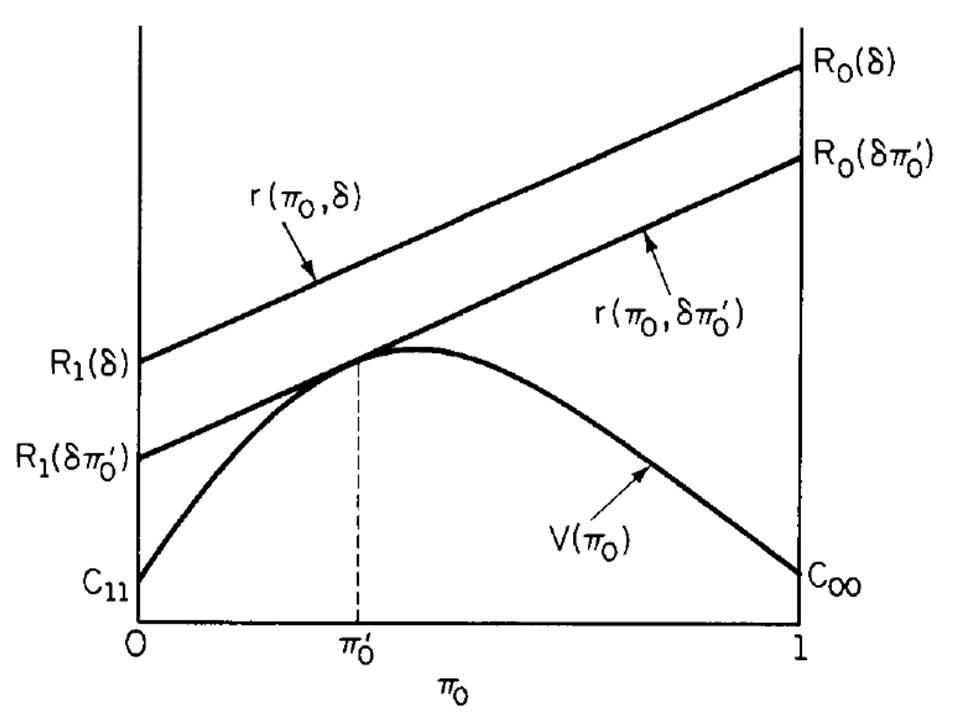
\includegraphics[width=0.9\linewidth]{Figures/minimax1}
	\caption[abc]{Illustration of the functions $r(\pi_0,\delta)~and~V(\pi_0)$}
	\label{fig:minimax1}
\end{figure}
To derive the Minimax rule, we first consider the unconditional risk for a given decision rule $\delta$ and a given prior for $H_0$, i.e $\pi_0 , \pi_0 \in [0,1]$. The average risk is given as:
\begin{equation}
r(\pi_0,\delta)=~\pi_0R_0(\delta)~+~(1-\pi_0)R_1(\delta), ~~~~\pi_0 \in [0,1]\\
\end{equation}
The unconditional risk function is shown in Fig:4. As can be seen, for a fixed $\delta$, the function $r(\pi_0,\delta)$ takes a value $R_1(\delta)~at~\pi_0=0~and~R_0(\delta)~at~\pi_0=1$. Thus, it is an affine function (\textit{An \textbf{affine function} is a function composed of a linear function plus a constant and its graph is a straight line}) which attains max values at the extrimities.
\begin{equation}
	\mathop {\max }\limits_{0 \le {\pi _0} \le 1} r({\pi _0},\delta ) = max\{ {R_0}(\delta ),{R_1}(\delta )\}
\end{equation}
\begin{figure}[h]
	\centering
	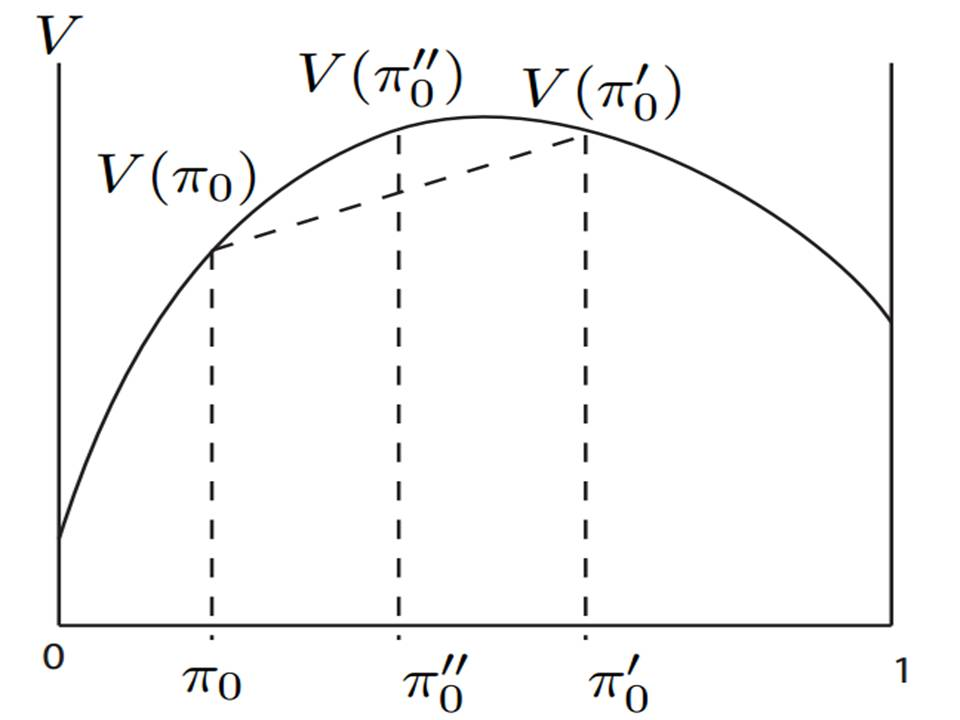
\includegraphics[width=0.7\linewidth]{Figures/concave}
	\caption{$V(\pi)$ as a concave function}
	\label{fig:concave}
\end{figure}
So, we have to design a decision rule that minimises the maximum value of the unconditional risk over all $\delta$.\\ 
Now, for each prior $\pi_0 \in~[0,1],$ let $\delta_{\pi_0}$ denote a Bayes rule corresponding to that prior, and let $V(\pi_0) = r(\pi_0,\delta_{\pi_0}) $; that is, $V(\pi_0)$ is the minimum possible Bayes risk for the prior $\pi_0$.
It can be proved that $V(\pi_0)$ is a continuous concave function of $\pi_0$ for $\pi_0 \in [0,1]$ with $V(0)=C_{11} ~and~ V(1)=C_{00}$. The proof is as follows:\\
\textbf{Claim: For any index set $\Delta$ the function \textbf{$V:[0,1] \to\mathcal R$} is a concave function}.\\ \\
A function is concave if, for any $\left\lbrace x,y\right\rbrace$ in the domain of \textit{f} and any $\alpha  \in [0,1],$
\begin{equation}
f(\alpha x + (1 - \alpha )y) \ge \alpha f(x) + (1 - \alpha )f(y).\\
\end{equation}
\begin{proof}
	 Let us denote a pair of priors as $\pi$ and $\pi'$ and a third prior $\pi''  = \alpha \pi  + (1 - \alpha )\pi'$.
We can write\\
\begin{align}
V(\pi'' ) &= \pi'' R({\delta _\pi'' })\\ \nonumber
&=\alpha \pi R({\delta _\pi'' }) + (1 - \alpha )\pi' R({\delta _\pi ''})
\end{align}
\begin{equation}
\ge \alpha V(\pi )) + (1 - \alpha )V(\pi' )
\end{equation}
Hence $V(\pi)$ is concave.\\ \\
\end{proof}
It can also readily be seen that $V(0)=C_{11}$ and $V(1)=C_{00}$.\\ \\
Suppose that $V(\pi_0)$ and $r(\pi_0,\delta)$ are as depicted in Fig 4. Also shown in Fig 4 is the line labelled $r({\pi _0},{\delta _{{\pi _0'}}})$, that is both parallel to $r({\pi _0},{\delta})$ as well as tangent to $V(\pi_0)$. For this case, $\delta$ cannot be the minimax rule because the risk line shown as $r({\pi _0},{\delta _{{\pi _0'}}})$  lies completely below $r({\pi _0},{\delta})$ and thus has a smaller maximum value. Since $r({\pi _0},{\delta _{{\pi _0'}}})$ touches $V(\pi_0)$ at $\pi_0 = \pi_0'$, $\delta _{{\pi _0'}}$ is a Bayes Rule for the prior $\pi_0'$. Since a similar tangent line can be drawn for any decision rule $\delta$, it is easily seen that only Bayes Rules can possibly be Minimax rules for Fig 4. \\
\begin{figure}[h]
	\centering
	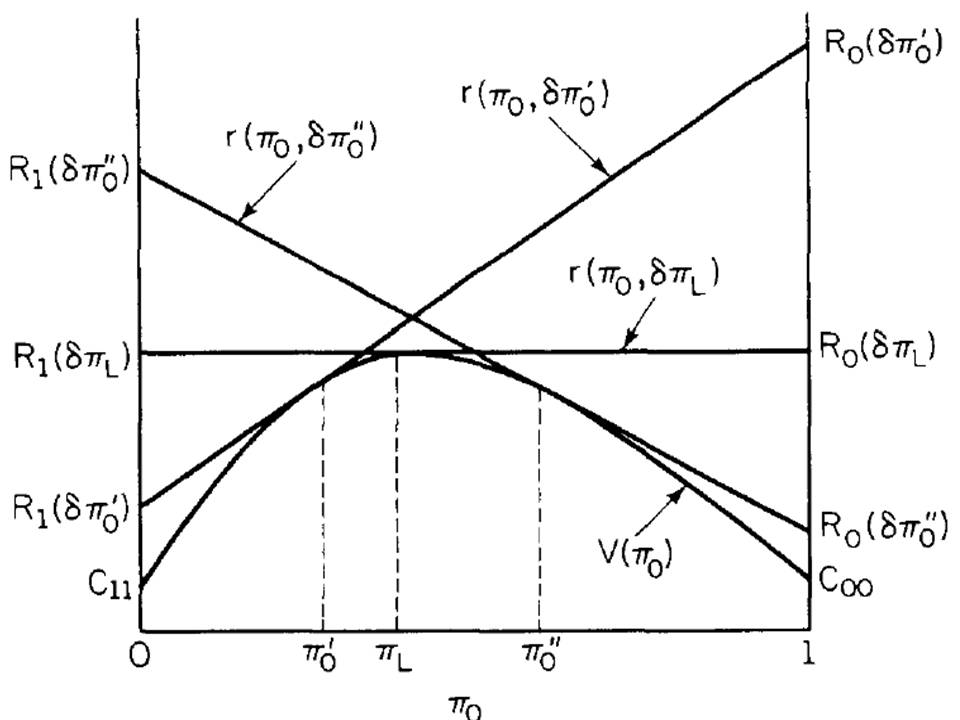
\includegraphics[width=0.7\linewidth]{Figures/minimax2}
	\caption{\textit{Illustartion of the Minimax Rule when V has an interior maximum}}
	\label{fig:minimax2}
\end{figure}
Moreover, by examination of Fig.6, we see that the Minimax rule for this case is a Bayes rule for the prior value $\pi_L$ that maximizes $V(\pi_0)$
over $\pi_0 \in [0,1]$. Note that for this prior we have that $r(\pi_0,\delta_{\pi_L})$ is constant over $\pi_0$, so,
\begin{equation}
max\{ {R_0}({\delta _{{\pi _L}}}),{R_1}({\delta _{{\pi _L}}})\}  = {R_0}({\delta _{{\pi _L}}}) = {R_1}({\delta _{{\pi _L}}})
\end{equation}  
The fact that $\delta_{\pi_L}$ is minimax follows from the Fig 6, since if $\pi_0' < \pi_L$, we have $max\{ {R_0}({\delta _{\pi_0'}}),{R_1}({\delta _{\pi_0'}})\}  = {R_0}({\delta _{{\pi _0'}}})>{R_0}({\delta _{{\pi _L}}})$, and if $\pi_0'' > \pi_L$, we have that
$max\{ {R_0}({\delta _{\pi_0''}}),{R_1}({\delta _{\pi_0''}})\}  = {R_1}({\delta _{{\pi _0''}}})>{R_1}({\delta _{{\pi _L}}})$, as depicted.
Because $\pi_L$ in Fig.6 maximizes the minimum Bayes risk, it is called
the \textbf{least-favourable prior}. Thus for this case a minimax decision rule is the Bayes rule for the least-favourable prior.
\begin{prop}
Suppose $\pi_L$ maximises $V(\pi_0)$ for $\pi_0 \in [0,1]$, then either $\pi_L=0$ or $R_1(\delta{\pi_L})=R_0(\delta{\pi_L})$ and then $\delta_{\pi_L}$ is a Minimax rule.
\end{prop} 
\begin{proof}
	Consider the case when $R_1(\delta{\pi_L})=R_0(\delta{\pi_L})$. We also know 
\begin{equation}
V({\pi _0}) = \mathop {\min }\limits_\delta  r({\pi _0},\delta ) = r({\pi _L},{\delta _{{\pi _L}}}).\\
\end{equation}
Now,\\
\begin{equation}
\mathop {\max }\limits_{{\pi _0} \in [0,1]} \mathop {\min }\limits_\delta  r({\pi _0},\delta ) = r({\pi _L},{\delta _{{\pi _L}}})=r({\pi _0},{\delta _{{\pi _L}}})
\end{equation}
\begin{equation}
\mathop {\max }\limits_{{\pi _0} \in [0,1]} \mathop {\min }\limits_\delta  r({\pi _0},\delta ) = \mathop {\max }\limits_{{\pi _0} \in [0,1]} r({\pi _0},{\delta _{{\pi _L}}}) \ge \mathop {\min }\limits_\delta  \mathop {\max }\limits_{{\pi _0} \in [0,1]} r({\pi _0},\delta )
\end{equation}

We can also say that
\begin{equation}
\mathop {\max }\limits_{{\pi _0} \in [0,1]} r({\pi _0},\delta ) \ge \mathop {\max }\limits_{{\pi _0} \in [0,1]} \mathop {\min }\limits_\delta  r({\pi _0},\delta )
\end{equation}
Indeed we have shown that 
\begin{equation}
r({\pi _L},{\delta _{{\pi _L}}}) = \mathop {\min }\limits_\delta  \mathop {\max }\limits_{{\pi _0} \in [0,1]} r(\pi ,\delta )
\end{equation}
\end{proof}
Now, $r(\pi,\delta_{\pi_0'})\geq V(\pi)$ since $V(\pi)$ minimises Bayes risk for all $\delta$. Also $r(\pi,\delta_{\pi_0'})$ is a straight line tangent to V at $\pi_0=\pi_0'$.\\
Hence, if V is differentiable,
\begin{equation}
V'(\pi ) = \frac{d}{{d\pi }}r(\pi ,{\delta _{{\pi _0'}}})\left| {_{\pi  = {\pi _0'}}} \right.
\end{equation}
\begin{equation}
~~~~~~~~= {R_0}({\delta _{{\pi _0'}}}) - {R_1}({\delta _{{\pi _0'}}})
\end{equation} 
Thus, under the condition of unknown priors, the Minimax rule considers the worst case scenario by taking the least favourable prior $\pi_L$ into account and further proceeds to minimise the maximum unconditional risk thus obtained.

\end{document}
